% 正文宋体小四
\documentclass[twoside,zihao=-4,UTF8]{bjfu}
%%%%%%%%%%%%%%%%%%%%%%%%%%%%%%%%%%%%%%%%%%%%%%%%%%%
% 汉语标题(此处的标题为页眉上的标题)
\bjfuTitle{请在此写上你的论文标题}
% 英语标题(此处的标题对应英文摘要页中的标题)
\bjfuTitleEn{Please text your english title here}

% 汉语摘要
% 注意在摘要结束后需要空一行,即右括号"}"要与摘要分隔开,避免行距变为单倍行距的bug
\bjfuAbstract{
分布式训练主要的应用场景就是例如当训练数据量较大时,单卡训练耗时过长,需要分布式训练技术提高训练效率;或者当单卡无法支持训练时,即单卡显存无法放下全量模型参数时,可使用分布式训练技术将模型参数等模型信息切分到多张卡或多台设备上,以保证模型可训练。简单来说无外乎两点:
\begin{itemize}
    \item 加快训练速度;
    \item 让单卡无法训练的模型可训练。
\end{itemize}

当下分布式训练主要有两种训练模型,第一种是集合通信模型,第二种是参数服务器模型。集合通信模型适用于CV/NLP相关的任务,参数服务器模型适用于CTR等相关的任务。这是因为一般来说CV/NLP相关的任务模型的参数都比较稠密,而搜索/推荐相关的任务模型的参数都比较稀疏。稠密参数(Dense\_Var)是指每个 step 都会更新的参数,比如 FC 的 Weight 参数。稀疏参数(Sparse\_Var)是指每个 step 不是必须更新的参数,如 Embedding 参数,只会更新当前 step 中涉及到的 key 的相应 value。

}

% 汉语关键字
\bjfuKeywords{计算机视觉,自然语言处理,语言/视觉大模型,分布式计算,高性能计算}

% 英文作者
\bjfuAuthorEn{Zhang San}
% 英文专业
\bjfuMajorEn{Mathematics}
% 英文指导老师
\bjfuSupervisorEn{Li Si}
% 英语摘要
\bjfuAbstractEn{
Please text your english abstract.
}

% 英语关键字
\bjfuKeywordsEn{Computer Vision, Natural Language Processing, Large Language/Vision Models, Distributed Computing, High Performance Computing}


%%%%%%%%%%%%%%%%%%%%%%%%%%%%%%%%%%%%%%%%%%%%%%%%%%%
\fancypagestyle{plain}{ \pagestyle{fancy} }
\begin{document}

% 注意!本模板采用直接插入pdf文件的方法导入封面和独创性声明等难以排版的页面,
% 请通过word(或其他软件)将封面、独创性声明和答辩委员会成员输出为pdf后,
% 通过\includepdf{}语句插入:

\includepdf[pages={1,2,3}]{src/statement.pdf}

\makeBjfuTitlePage
\zihao{-4}

\section{章标题}\label{sec:introduction}
\fancyhead[CO]{\zihao{5}\CJKfamily{zhsong}请手动改成你的章标题}
\renewcommand{\headrulewidth}{0.8pt}
\fancyhead[CE]{\zihao{5}\CJKfamily{zhsong}\bjfuTitleString}

\subsection{节标题}\label{sec:background}

\subsubsection{二级节标题}

\section{常用LaTeX命令参考样式}
\fancyhead[CO]{\zihao{5}\CJKfamily{zhsong}也请手动改成你的章标题}
\renewcommand{\headrulewidth}{0.8pt}
\fancyhead[CE]{\zihao{5}\CJKfamily{zhsong}\bjfuTitleString}

\subsection{参考文献插入的参考样式}
使用BibTeX格式参考文献,使用命令\verb+\cite+即可引用,如:自然语言处理中的Attention is All You Need~\cite{vaswani2017attention},分布式计算中NVIDIA的Megatron系列论文~\cite{shoeybi2019megatron, narayanan2021efficient, korthikanti2023reducing}....

\subsection{罗列要点的参考样式}
本研究的主要创新点和贡献可总结为以下五点:
\begin{itemize}
    \item 也可以通过;
    \item itemize实现;
    \item 罗列;
\end{itemize}

\subsection{图片插入的参考样式}
SVM有着优良的分类性能,从\autoref{fig:demo_of_SVM}中可以看出,SVM能够准确地识别出不同类别的数据,并给出合理的的决策边界(图中黑色实线)。
\begin{figure}[h]
	\center
	% Use the relevant command to insert your figure file.
	% For example, with the graphicx package use
	\subcaptionbox{\text{传统软间隔SVM(线性核)} \label{fig:demo_of_linear_SVM}}
	{
		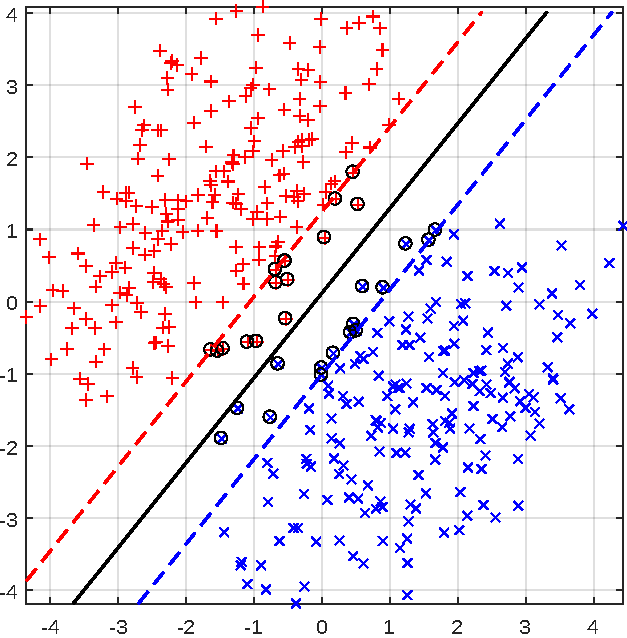
\includegraphics[width=0.45\textwidth]{figs/demo_of_linear_SVM_cropped.pdf}
	}
	\subcaptionbox{\text{非线性软间隔SVM(高斯核)} \label{fig:demo_of_kernel_SVM}}
	{
		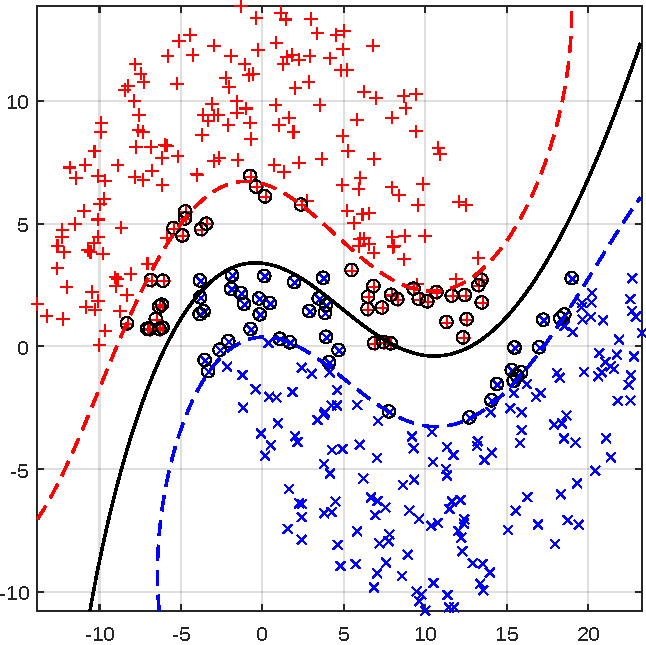
\includegraphics[width=0.458\textwidth]{figs/demo_of_kernel_SVM_cropped.pdf}
	} 
	\bicaption{线性SVM和非线性SVM在不同数据类型下的决策边界 
	\vspace{1.1ex}}{Classification 
	boundaries of linear SVM and nonlinear SVM under different data 
	distributions}
	\label{fig:demo_of_SVM}       % Give a unique label
\end{figure}

\subsection{表格插入的参考样式}
为了简便起见,\autoref{tab:notations}总结了本论文出现的主要数学符号。
\begin{table*}[h]
	\renewcommand\arraystretch{1.25}
	\centering
	\bicaption{符号对照说明表 \vspace{1.1ex}}{Table of notations}
	\label{tab:notations}
	\begin{tabular}{p{160pt}p{260pt}}
		\toprule[1.2pt]
		\textbf{符号} & \textbf{说明} \\
		\midrule
		$(x_{i}, y_{i})$ & 第$i$个单视角训练样本及其标签 $y_{i}$\\
		$(x_{i}^{A}, x_{i}^{B}, y_{i})$ & 第$i$个多视角训练样本及其标签 $y_{i}$\\
		$l^{+}$, $l^{-}$ & 正类(负类)训练样本的个数 \\
		$\boldsymbol{c}_{\pm}^{A},  \  \boldsymbol{c}_{\pm}^{B}$ & 
		分别对应于视角A和视角B的正类(负类)超球球心 \\
		$R_{\pm}^{A} , \ R_{\pm}^{B} $ & 
		分别对应于视角A和视角B的正类(负类)超球半径 \\
		$ \langle x_{i}, \ x_{j} \rangle$ & 
		向量$x_{i}$和$x_{j}$的内积,或写为$x_{i}^{\top}x_{j}$ \\
		$\varphi( \ \cdot \ ), \  \varphi_{A}( \ \cdot \ ), \   \varphi_{B}( \ 
		\cdot \ )$  & 将原空间
		映射到高维特征空间的正定核映射 \\
		$k(x_{i}, x_{j})$ & 传统单视角中的核函数 $ \langle 
		\varphi(x_{i}), \ \varphi(x_{j}) \rangle$ \\
		$k^{A}(x_{i}^{A}, x_{j}^{A})$ & A视角核函数 $ \langle 
		\varphi_{A}(x_{i}^{A}), \ \varphi_{A}(x_{j}^{A}) \rangle$\\
		$ k^{B}(x_{i}^{B}, x_{j}^{B})$ & 
		B视角核函数$ \langle
		\varphi_{B}(x_{i}^{B}), \ \varphi_{B}(x_{j}^{B}) \rangle $\\
		$\left\| \ \cdot \ \right\|_{p}$ & 向量的$l_p$-范数 
		(如果$p$省略,则默认取$l_2$-范数) \\
		$\boldsymbol{Q}_{(\cdot \times \cdot)}$ & 大写黑体西文字符表示矩阵,其规模
		可
		见下标 \\
		$\boldsymbol{q}_{(\cdot \times \cdot)}$ & 小写黑体西文字符表示列向量,其长
		度可见下标 \\
		$diag(\cdot)$ & 表示取矩阵对角线元素的运算符\\
		\bottomrule[1.2pt]
	\end{tabular}
\end{table*}

\subsection{公式输入的参考样式}\label{sec:svm}
支持向量机(SVM)是机器学习的经典算法,它的优化学习目标是在两类样本点之间寻求最大间隔和
最小误
差的权衡。令$\mathscr{X} \in 
{{R}^{{{d}}}}$为$d$维的样本属性空间,$\mathscr{Y}=\left\{ 
-1,+1 
\right\}$为样本标签空间。考虑一个有监督二分类问题,其训练样本集表示为$T=\left\{
\left( x_{i},{{y}_{i}} \right)\left| x_{i}\in \mathscr{X},{{y}_{i}}\in 
\mathscr{Y} \right. \right\}_{i=1}^{l}$,SVM将在样本空间中寻找能将两类样本点以最大
间隔分开的决策超平面:
\begin{equation}
	\langle \boldsymbol{\omega}, \varphi (x) \rangle + b = 0 ,
\end{equation}
其中,${\boldsymbol{\omega}}$和$b$分别表示样本属性空间中决策超平面的法向量与
偏置项。

SVM的原问题是:
\begin{equation}
	\begin{aligned}
		\underset{\boldsymbol{\omega},b,\xi}{\mathop{\min }} & \quad 
		\cfrac{1}{2}{{\left\| \boldsymbol{\omega} 
		\right\|}^{2}} + C \sum\limits_{i=1}^{l}{{{\xi }_{i}}} \\ 
		s.t. & \quad {{y}_{i}}\left( \langle \boldsymbol{\omega}, \varphi 
		(x_{i}) 
		\rangle + b \right)\le 1-{{\xi }_{i}}, \\
		& \quad \xi_{i} \ge 0, \ i = 1,2,...,l,
	\end{aligned}
\end{equation}
其中,${{\varphi}(.)}$表示任意正定核映射,$C$是松弛变量的惩罚参数,且$C>0$。

在SVM的目标函数中,正则化项$\cfrac{1}{2}{{\left\| \boldsymbol{\omega} 
\right\|}^{2}}$旨在最大化超平面$\langle \boldsymbol{\omega}, \varphi (x) \rangle 
+ b = +1$和$\langle \boldsymbol{\omega}, \varphi (x) \rangle + b = 
-1$之间的距离,起到结构风险最小化的作用;而约束条件要求样本点在两条超平面之外,若落入
超平面之间,则引入松弛变量$\left\{ {{\xi }_{i}} 
\right\}_{i=1}^{l}$来使得约束成立;目标函数的第二项是最小化松弛变量之和,旨
在尽可能地避免样本落入间隔内,起到经验风险最小化的作用;惩罚因子$C$用于权衡目标函数的
结构风险和经验风险。

SVM的对偶问题是:
\begin{equation}
	\begin{aligned}
		\underset{\alpha}{\min} & \quad 
		\cfrac{1}{2}\underset{i=1}{\overset{l}{\mathop \sum }} 
		\underset{j=1}{\overset{l}{\mathop \sum }}{{\alpha }_{i}}{{\alpha}_{j}}{{y}_{i}}{{y}_{j}}k(x_{i},x_{j}) - 
		\underset{i=1}{\overset{l}{\mathop \sum }}{{\alpha }_{i}} \\
		s.t. & \quad \underset{i=1}{\overset{m}{\mathop \sum }}{{\alpha}_{i}}{{y}_{i}}=0,  \\
		& \quad 0 \le {{\alpha }_{i}}\le C, \ i=1,2,\ldots ,l.  \\
	\end{aligned} 
\end{equation}
通过对偶问题求解出$\boldsymbol{\omega}$和$b$后,可得到SVM对未知样本$x$的决策函数:
\begin{equation}
	f(x) = sign\left(\langle \boldsymbol{\omega}, \varphi(x) \rangle + b\right).
\end{equation}


\subsection{普通表格的插入样式}
\begin{table*}[h!]
    \begin{center}
    \bicaption{注意力类型研究 \vspace{1ex}}{Ablation study of Attention Type.}
    \label{tab:bmtransformer_ablation_attention_type}
    \begin{tabular}{llc}
    \toprule[1pt]
    Attention Type                                            &  Information Exchange        &  mIoU (\%)      \\
    \midrule
    Window Attention                                          &  Local                 & 69.4           \\
    Window Attention\textdagger                               &  Local                  & 70.1           \\
    \midrule
    Region-Local Attention                                    & Regional-Local          & 71.0           \\
    \midrule
    Broadcast-and-Mixing                   & Global-Regional-Local   & \textbf{71.9}          \\
    \bottomrule[1pt]
    \end{tabular}
    \end{center}
\end{table*}

\subsection{长表格插入的参考样式}
\newcommand{\tabincell}[2]{\begin{tabular}{@{}#1@{}}#2\end{tabular}} 
{\zihao{5}
\begin{flushleft}
	\begin{longtable}[h]{p{55pt}p{50pt}p{50pt}p{50pt}p{50pt}p{50pt}p{50pt}}
		\bicaption{AwA数据集性能对比(Accu. $\pm$ std.) \vspace{1.1ex}}{Benchmark 
		results on AwA 
		data sets (Accu. $\pm $ std.)}
		\label{tab: AwA_res}\\
		\toprule[1.0pt]
		\endfirsthead
		\toprule[1.0pt]
		\multicolumn{7}{l}{续 \autoref{tab: AwA_res}}\\
		\midrule
		\endhead
		\bottomrule[1.0pt]
		\endfoot
		\tabincell{l}{\textbf{数据集名称} \\ {}} & \tabincell{l}{\textbf{SVM-2K} 
		\\ Accu. (\%) } & 
		\tabincell{l}{\textbf{MVMED} \\ Accu. (\%) } &  
		\tabincell{l}{\textbf{MvTwSVMs} \\ Accu. 
		(\%) } &
		\tabincell{l}{\textbf{MvNPSVM} \\ Accu. (\%) }& 
		\tabincell{l}{\textbf{Ours} \\ 
		\textbf{Accu. (\%)} } &
		\tabincell{l}{\textbf{Ours-2C} \\ \textbf{Accu. (\%)} }\\
		\midrule
		chi vs. pan & 68.15$\pm$4.81 & 47.99$\pm$4.48 & 68.42$\pm$2.31 & 
		85.57$\pm$0.83 & 86.56$\pm$0.71 & \textbf{88.70$\pm$0.68} \\
		chi vs. leo & 75.13$\pm$4.40 & 47.40$\pm$2.91 & 76.40$\pm$0.99 & 
		84.39$\pm$1.64 & 85.09$\pm$0.77 & \textbf{87.03$\pm$0.62} \\
		chi vs. per & 65.43$\pm$2.60 & 83.74$\pm$0.72 & 75.70$\pm$1.03 & 
		\textbf{85.10$\pm$0.78} & 84.13$\pm$0.71 & 84.29$\pm$0.61 \\
		chi vs. pig & 78.33$\pm$2.47 & 47.18$\pm$3.31 & 66.94$\pm$2.02 & 
		82.34$\pm$0.56 & \textbf{83.81$\pm$1.04} & 83.03$\pm$0.74 \\
		chi vs. hip & 45.58$\pm$1.81 & 49.57$\pm$4.41 & 71.71$\pm$1.69 & 
		81.70$\pm$1.12 & 80.88$\pm$0.66 & \textbf{84.07$\pm$1.12} \\
		chi vs. hum & 90.73$\pm$2.14 & 94.81$\pm$0.56 & 88.10$\pm$0.53 & 
		94.88$\pm$0.54 & 93.82$\pm$0.65 & \textbf{95.94$\pm$1.03} \\
		chi vs. rac & 83.43$\pm$1.33 & 46.86$\pm$2.81 & 63.65$\pm$1.65 & 
		83.31$\pm$0.75 & 84.69$\pm$0.99 & \textbf{84.95$\pm$1.11} \\
		chi vs. rat & 64.90$\pm$1.59 & 76.18$\pm$1.01 & 66.41$\pm$1.95 & 
		79.48$\pm$1.08 & \textbf{81.90$\pm$1.10} & 79.73$\pm$0.96 \\
		chi vs. seal & 82.05$\pm$1.37 & 84.04$\pm$0.72 & 74.51$\pm$1.25 & 
		47.68$\pm$3.64 & 86.49$\pm$0.76 & \textbf{88.14$\pm$0.58} \\
		pan vs. leo & 82.00$\pm$2.36 & 82.46$\pm$0.66 & 69.17$\pm$1.83 & 
		\textbf{88.97$\pm$0.97} & 87.07$\pm$0.89 & 88.09$\pm$0.64 \\
		pan vs. per & 56.90$\pm$0.76 & 87.73$\pm$0.76 & 80.56$\pm$1.10 & 
		89.27$\pm$0.74 & \textbf{89.45$\pm$0.71} & 88.17$\pm$0.35 \\
		pan vs. pig & 63.21$\pm$1.29 & 77.91$\pm$1.66 & 61.43$\pm$2.13 & 
		82.53$\pm$0.99 & \textbf{82.65$\pm$0.74} & 80.79$\pm$1.24 \\
		pan vs. hip & 75.56$\pm$0.78 & 83.65$\pm$0.75 & 68.94$\pm$1.79 & 
		88.51$\pm$1.03 & 85.72$\pm$0.98 & \textbf{89.04$\pm$0.66} \\
		pan vs.hum & 49.22$\pm$4.23 & 96.03$\pm$0.49 & 89.00$\pm$1.14 & 
		96.26$\pm$0.33 & 96.14$\pm$0.34 & \textbf{97.07$\pm$0.47} \\
		pan vs. rac & 76.75$\pm$2.50 & 84.56$\pm$1.14 & 61.44$\pm$1.00 & 
		87.26$\pm$1.19 & \textbf{87.90$\pm$1.00} & 87.31$\pm$0.91 \\
		pan vs. rat & 64.26$\pm$1.06 & 82.62$\pm$1.22 & 66.83$\pm$2.66 & 
		85.40$\pm$0.99 & \textbf{88.00$\pm$0.93} & 86.21$\pm$1.05 \\
		pan vs. sea & 80.50$\pm$1.40 & 87.06$\pm$0.64 & 74.77$\pm$2.19 & 
		88.59$\pm$0.84 & 88.66$\pm$0.66 & \textbf{90.23$\pm$0.70} \\
		leo vs. per & 52.16$\pm$4.36 & 50.66$\pm$7.14 & 85.70$\pm$0.76 & 
		\textbf{90.91$\pm$0.69} & 90.56$\pm$0.31 & 90.07$\pm$0.45 \\
		leo vs. pig & 65.01$\pm$1.10 & 47.10$\pm$3.70 & 72.45$\pm$1.28 & 
		78.19$\pm$0.87 & \textbf{78.99$\pm$1.11} & 78.42$\pm$1.21 \\
		leo vs. hip & 73.44$\pm$0.86 & 82.42$\pm$0.87 & 78.38$\pm$1.03 & 
		82.94$\pm$1.12 & 84.14$\pm$1.06 & \textbf{84.37$\pm$0.58} \\
		leo vs. hum & 85.05$\pm$3.77 & 95.57$\pm$0.61 & 91.65$\pm$0.29 & 
		95.25$\pm$0.40 & 95.13$\pm$0.19 & \textbf{95.94$\pm$0.25} \\
		leo vs. rac & 56.29$\pm$5.19 & 48.31$\pm$3.56 & 60.82$\pm$3.52 & 
		\textbf{77.32$\pm$1.46} & 75.29$\pm$1.11 & 76.39$\pm$1.46 \\
		leo vs. rat & 59.85$\pm$0.84 & 83.91$\pm$0.64 & 76.71$\pm$1.40 & 
		75.15$\pm$6.60 & 83.13$\pm$0.56 & \textbf{83.96$\pm$0.89} \\
		leo vs. sea & 62.94$\pm$4.96 & 87.26$\pm$0.67 & 84.37$\pm$0.71 & 
		\textbf{88.46$\pm$0.52} & 88.24$\pm$0.84 & 87.72$\pm$1.14 \\
		per vs. pig & 66.00$\pm$6.37 & 78.24$\pm$0.84 & 73.93$\pm$0.96 & 
		79.06$\pm$0.99 & \textbf{79.50$\pm$1.03} & 79.24$\pm$1.63 \\
		per vs. hip & 72.66$\pm$3.78 & 83.85$\pm$0.79 & 78.37$\pm$1.00 & 
		85.66$\pm$0.50 & 86.02$\pm$1.21 & \textbf{86.54$\pm$1.15} \\
		per vs. hum & 91.89$\pm$0.88 & 88.46$\pm$0.86 & 83.42$\pm$0.78 & 
		92.19$\pm$0.42 & 91.41$\pm$0.29 & \textbf{95.91$\pm$0.42} \\
		per vs. rac & 47.42$\pm$5.11 & 47.78$\pm$3.58 & 73.39$\pm$1.40 & 
		85.84$\pm$0.69 & 84.06$\pm$0.75 & \textbf{87.43$\pm$0.83} \\
		per vs. rat & 66.52$\pm$3.26 & 68.18$\pm$1.34 & 61.35$\pm$1.70 & 
		68.27$\pm$1.69 & 69.29$\pm$0.78 & \textbf{69.76$\pm$1.28} \\
		per vs. sea & 78.52$\pm$1.82 & 84.72$\pm$1.08 & 75.11$\pm$0.82 & 
		\textbf{85.30$\pm$1.17} & 84.01$\pm$0.76 & 83.35$\pm$0.68 \\
		pig vs. hip & 71.36$\pm$2.02 & 70.94$\pm$1.44 & 64.53$\pm$1.19 & 
		71.87$\pm$0.82 & 72.29$\pm$1.14 & \textbf{72.43$\pm$1.29} \\
		pig vs. hum & 90.11$\pm$1.29 & 91.26$\pm$0.67 & \textbf{94.15$\pm$0.40} 
		& 93.01$\pm$0.42 & 91.50$\pm$0.40 & 92.76$\pm$0.51 \\
		pig vs. rac & 72.32$\pm$1.94 & 73.88$\pm$1.49 & 58.46$\pm$0.81 & 
		80.98$\pm$1.36 & \textbf{80.96$\pm$0.85} & 80.07$\pm$1.20 \\
		pig vs. rat & 57.73$\pm$2.40 & 48.59$\pm$4.62 & 55.90$\pm$2.55 & 
		68.89$\pm$1.96 & 71.46$\pm$1.39 & \textbf{72.22$\pm$0.85} \\
		pig vs. sea & 75.08$\pm$0.83 & 78.03$\pm$1.02 & 67.10$\pm$2.11 & 
		\textbf{78.97$\pm$0.91} & 77.71$\pm$1.14 & 78.70$\pm$0.72 \\
		hip vs. hum & 81.40$\pm$1.05 & 88.15$\pm$1.07 & 75.67$\pm$1.54 & 
		\textbf{88.45$\pm$0.87} & 88.04$\pm$0.47 & 88.36$\pm$0.74 \\
		hip vs. rac & 79.20$\pm$1.11 & 79.61$\pm$0.83 & 69.54$\pm$1.23 & 
		\textbf{81.60$\pm$1.12} & 81.57$\pm$1.03 & 80.53$\pm$1.31 \\
		hip vs. rat & 59.95$\pm$0.85 & 47.85$\pm$2.67 & 67.42$\pm$2.82 & 
		75.01$\pm$1.07 & \textbf{79.08$\pm$1.21} & 77.19$\pm$0.97 \\
		hip vs. sea & 54.37$\pm$4.15 & 70.24$\pm$1.09 & 60.20$\pm$2.99 & 
		\textbf{70.95$\pm$1.35} & 69.85$\pm$0.90 & 69.96$\pm$1.26 \\
		hum vs. rac & 63.09$\pm$4.41 & 90.90$\pm$0.66 & 86.24$\pm$1.17 & 
		92.34$\pm$0.50 & 92.69$\pm$0.56 & \textbf{93.81$\pm$0.57} \\
		hum vs. rat & 84.48$\pm$0.67 & 88.22$\pm$0.67 & 81.62$\pm$0.81 & 
		\textbf{89.94$\pm$0.55} & 87.81$\pm$0.76 & 89.27$\pm$0.56 \\
		hum vs. sea & 84.91$\pm$1.54 & 83.99$\pm$0.63 & 74.72$\pm$1.43 & 
		85.08$\pm$0.72 & 85.28$\pm$0.86 & \textbf{85.37$\pm$0.59} \\
		rac vs. rat & 57.80$\pm$1.62 & 71.74$\pm$0.91 & 65.97$\pm$1.47 & 
		46.78$\pm$2.09 & \textbf{76.12$\pm$1.13} & 76.10$\pm$1.10 \\
		rac vs. sea & 52.77$\pm$5.45 & 85.72$\pm$0.79 & 76.25$\pm$1.34 & 
		\textbf{86.29$\pm$0.50} & 85.58$\pm$0.82 & 85.66$\pm$0.55 \\
		rat vs. sea & 66.59$\pm$2.30 & 74.66$\pm$0.98 & 66.22$\pm$1.77 & 
		75.65$\pm$1.07 & 76.26$\pm$1.04 & \textbf{76.58$\pm$0.99} \\
		\midrule
		平均准确率 & 69.58 & 74.45 & 72.97 & 82.26 & 83.98 & \textbf{84.46} \\
		平均耗时 & 3.03  & 63.64 & 0.98 & 5.32 & \textbf{0.20} & 2.07 \\
		平均排名 & 5.18  & 4.18  & 5.07  & 2.42  & 2.38  & \textbf{1.78}
	\end{longtable}
\end{flushleft}}

\subsection{定义、定理、引理与证明环境的参考样式}
\newtheorem{lemma}{引理}
\begin{lemma}[$\boldsymbol{\pi}$的稀
	疏性] \label{lemma:sparsity}
	假设\eqref{eq:ppmvthsvm1}的解为$\boldsymbol{c}_{+}^{A*}, 
	\boldsymbol{c}_{+}^{B*},R_{+}^{{{A}^{2}*}},R_{+}^{{{B}^{2}*}}$,其对偶问题
	\eqref{eq:dpmvthsvm1}的最优解为$\boldsymbol{\pi}^{*} 
	=\left(\boldsymbol{\alpha 
	}_{+}^{A\top*},\boldsymbol{\alpha }_{+}^{B\top*},\boldsymbol{\beta 
	}^{+\top*},\boldsymbol{\beta }^{-\top*} 
	\right)^{\top}$,则$\forall i \in 
	I^{+}$,多视角训练样本$\boldsymbol{x}_{i} = 
	\left\{x_{i}^{A},x_{i}^{B}\right\}$和$\boldsymbol{\pi}^{*}$
	满足如下关系:
	
样本的$A$视角特征$x_{i}^{A}$和$\boldsymbol{\alpha}_{+}^{A*}$之间满足:
	\begin{align}\ 
	&  x_{i}^{A} \in \mathcal{R}_{+}^{A} = \left\{x^{A} \left| {{\left\| 
	{{\varphi 
	}_{A}}( x^{A} )-\boldsymbol{c}_{+}^{A*} 
	\right\|}^{2}} < R_{+}^{{{A}^{2}*}} \right. \right\} \Rightarrow 
	\alpha_{i}^{A*} = 0, \\
	& x_{i}^{A} \in \mathcal{E}_{+}^{A} = \left\{x^{A} \left| {{\left\| 
	{{\varphi 
				}_{A}}( x^{A} )-\boldsymbol{c}_{+}^{A*} 
			\right\|}^{2}} = R_{+}^{{{A}^{2}*}} \right. \right\} \Rightarrow 
	\alpha_{i}^{A*} \in \left[0, \cfrac{c_{1}^{A}}{l^{+}}\right], \\
	& x_{i}^{A} \in \mathcal{L}_{+}^{A} = \left\{x^{A} \left| {{\left\| 
	{{\varphi 
				}_{A}}( x^{A} )-\boldsymbol{c}_{+}^{A*} 
			\right\|}^{2}} > R_{+}^{{{A}^{2}*}} \right. \right\} \Rightarrow 
	\alpha_{i}^{A*} = \cfrac{c_{1}^{A}}{l^{+}}, 
	\end{align}

样本的$B$视角特征$x_{i}^{B}$和$\boldsymbol{\alpha}_{+}^{B*}$之间满足:
\begin{align}\ 
	&  x_{i}^{B} \in \mathcal{R}_{+}^{B} = \left\{x^{B} \left| {{\left\| 
			{{\varphi 
				}_{B}}( x^{B} )-\boldsymbol{c}_{+}^{B*} 
			\right\|}^{2}} < R_{+}^{{{B}^{2}*}} \right. \right\} \Rightarrow 
	\alpha_{i}^{B*} = 0, \\
	& x_{i}^{B} \in \mathcal{E}_{+}^{B} = \left\{x^{B} \left| {{\left\| 
			{{\varphi 
				}_{B}}( x^{B} )-\boldsymbol{c}_{+}^{B*} 
			\right\|}^{2}} = R_{+}^{{{B}^{2}*}} \right. \right\} \Rightarrow 
	\alpha_{i}^{B*} \in \left[0, \cfrac{c_{1}^{B}}{l^{+}}\right], \\
	& x_{i}^{B} \in \mathcal{L}_{+}^{B} = \left\{x^{B} \left| {{\left\| 
			{{\varphi 
				}_{B}}( x^{B} )-\boldsymbol{c}_{+}^{B*} 
			\right\|}^{2}} > R_{+}^{{{B}^{2}*}} \right. \right\} \Rightarrow 
	\alpha_{i}^{B*} = \cfrac{c_{1}^{B}}{l^{+}}, 
\end{align}

多视角样本$\boldsymbol{x}_{i} 
=\left\{x_{i}^{A},x_{i}^{B}\right\}$和$\boldsymbol{\beta}^{+*},\boldsymbol{\beta}^{-*}$
之间满足:
\begin{align}
	\boldsymbol{x}_{i} & \in \mathcal{B}^{+} = \left\{\boldsymbol{x} \left| 
	{{\left\| 
	{{\varphi }_{A}}( x^{A})-\boldsymbol{c}_{+}^{A*} 
	\right\|}^{2}}-R_{+}^{{{A}^{2}*}} - {{\left\|{{\varphi }_{B}}( x^{B} 
	)-\boldsymbol{c}_{+}^{B*} \right\|}^{2}}+R_{+}^{{{B}^{2}*}}  > \epsilon  
	\right. 
	\right\} \nonumber \\ 
	& \Rightarrow \beta_{i}^{+*} = D_{1},\beta_{i}^{-*} = 0, \\
	\boldsymbol{x}_{i} & \in \mathcal{E}^{+} = \left\{\boldsymbol{x} \left| 
	{{\left\| 
			{{\varphi }_{A}}( x^{A})-\boldsymbol{c}_{+}^{A*} 
			\right\|}^{2}}-R_{+}^{{{A}^{2}*}} - {{\left\|{{\varphi }_{B}}( 
			x^{B} 
			)-\boldsymbol{c}_{+}^{B*} \right\|}^{2}}+R_{+}^{{{B}^{2}*}}  = 
			\epsilon  
	\right. 
	\right\} \nonumber \\ 
	& \Rightarrow \beta_{i}^{+*} = D_{1},\beta_{i}^{-*} = 0, \\
	\boldsymbol{x}_{i} & \in \mathcal{E} = \left\{\boldsymbol{x} \left| 
	\quad
	\left|
	{{\left\| 
			{{\varphi }_{A}}( x^{A})-\boldsymbol{c}_{+}^{A*} 
			\right\|}^{2}}-R_{+}^{{{A}^{2}*}} - {{\left\|{{\varphi }_{B}}( 
			x^{B} 
			)-\boldsymbol{c}_{+}^{B*} \right\|}^{2}}+R_{+}^{{{B}^{2}*}} \right|  
			< \epsilon  
	\right. 
	\right\} \nonumber \\ 
	& \Rightarrow \beta_{i}^{+*} =0,\beta_{i}^{-*} = 0, \\
	\boldsymbol{x}_{i} & \in \mathcal{E}^{-} = \left\{\boldsymbol{x} \left| 
	{{\left\| {{\varphi }_{B}}( x^{B})-\boldsymbol{c}_{+}^{B*} 
	\right\|}^{2}}-R_{+}^{{{B}^{2}*}} - {{\left\|{{\varphi }_{A}}( 
	x^{A} )-\boldsymbol{c}_{+}^{A*} \right\|}^{2}}+R_{+}^{{{A}^{2}*}} = 
	\epsilon  
	\right. 
	\right\} \nonumber \\ 
	& \Rightarrow \beta_{i}^{+*} = 0,\beta_{i}^{-*} = \left[0, D_{1}\right], \\
	\boldsymbol{x}_{i} & \in \mathcal{B}^{-} = \left\{\boldsymbol{x} \left| 
	{{\left\| {{\varphi }_{B}}( x^{B})-\boldsymbol{c}_{+}^{B*} 
			\right\|}^{2}}-R_{+}^{{{B}^{2}*}} - {{\left\|{{\varphi }_{A}}( 
			x^{A} )-\boldsymbol{c}_{+}^{A*} \right\|}^{2}}+R_{+}^{{{A}^{2}*}} 
			> 
	\epsilon  
	\right. 
	\right\} \nonumber \\ 
	& \Rightarrow \beta_{i}^{+*} = 0,\beta_{i}^{-*} = D_{1}, 
\end{align}
\end{lemma}
进一步地,在{\heiti 命题}和{\heiti 引理}\ref{lemma:sparsity}成立的
条件下,我们有关于$\boldsymbol{\beta}^{+*},\boldsymbol{\beta}^{-*}$的进一步推论:
\newtheorem{corollary}{推论}
\begin{corollary}
	当参数$\epsilon>0$时,令$\boldsymbol{u}^{-*} = 
	\boldsymbol{\beta}^{+*} - 
	\boldsymbol{\beta}^{-*}$,多视角样本$\boldsymbol{x}_{i} 
	=\left\{x_{i}^{A},x_{i}^{B}\right\}$和$\boldsymbol{u}^{-*}$
	之间满足:
\end{corollary}

\newtheorem{definition}{定义}
\begin{definition}[多视角边界误差点(multi-view margin errors, MEs)] 多视角边界
误差点指的是,该样本点在所有视角上,其
特征均在超球外,即$\boldsymbol{x}_{i} = \left\{x_{i}^{A},x_{i}^{B}\right\} \in 
\mathcal{L}_{+}^{A} \cap \mathcal{L}_{+}^{B}$。该类样本点的集合(MEs)可表述为:
	\begin{equation}
		\textit{MEs} = \left\{\boldsymbol{x}_{i} = 
		\left\{x_{i}^{A},x_{i}^{B}\right\} \left| 
		\|\varphi(x_{i}^{A}) - \boldsymbol{c}_{+}^{A*}\| > R_{+}^{A^2*} \ 
		\& \ 
		\|\varphi(x_{i}^{B}) - \boldsymbol{c}_{+}^{B*}\| > R_{+}^{B^2*} \right. 
		, i \in I^{+}
		\right\}.
	\end{equation}
\end{definition}

\begin{proof}
	\begin{align}
		&\sum\limits_{i\in {{MEs}}}{\left( \alpha_{i}^{A}+\alpha _{i}^{B} 
			\right)} \le \sum\limits_{i\in {{I}^{+}}}{\left( 
			\alpha_{i}^{A}+\alpha _{i}^{B} 
		\right)}=\sum\limits_{i\in {\textit{CVs}}}{\left( \alpha_{i}^{A}+\alpha 
		_{i}^{B} \right)}=2 \nonumber \\
		\Rightarrow & |\textit{MEs}|\cfrac{c_{1}^{A}+c_{1}^{B}}{l^{+}} \le 2 
		\le 
		|\textit{CVs}|\cfrac{c_{1}^{A}+c_{1}^{B}}{l^{+}} \nonumber \\
		\Rightarrow & \cfrac{|\textit{MEs}|}{l^{+}} \le 
		\cfrac{2}{c_{1}^{A}+c_{1}^{B}} \le 
		\cfrac{|\textit{CVs}|}{l^{+}} \Rightarrow \ {|\textit{MEs}|} \le 
		\cfrac{2{l^{+}}}{c_{1}^{A}+c_{1}^{B}} \le 
		{|\textit{CVs}|} .\nonumber
	\end{align}
\end{proof}


\subsection{算法伪代码的参考样式}
算法环境可以使用algorithm2e宏包(输入注释等非算法包命令可支持中文)。如下为添加了自适应梯度裁剪(Adaptive Gradient Clipping)方法~\cite{brock2021high}的AdamW~\cite{loshchilov2017decoupled}优化器伪代码:

\begin{algorithm*}[!t]
    \SetAlgoLined
    \KwIn{Parameter vector to optimize $w$; objective function $\mathcal{L}$; learning rate schedule $\eta_t$; initial moving averages $v_0 = 0, u_0 = 0$; exponential moving average parameters {$\beta_1, \beta_2$}; weight decay $\lambda$; regularization constants $\epsilon$.}
    \vspace{1mm}
    \KwIn{AGC hyperparameters: clipping threshold $\lambda$.}
    \vspace{1mm}

    \While{$w_t$ not converge}{
    \textbf{Compute} $g_t$ = $\frac{\partial \mathcal{L}(w_t)}{\partial w_t}$ $\to$ \text{obtain stochastic gradient.} \\[0.5em]
    \textbf{apply adaptive gradient clipping} \\[0.5em]
    \textcolor{blue}{$h_{t, i} = \min \{\frac{\lambda \|w_{t, i}\|}{g_{t, i}}, 1.0\}, \quad i \in |w|$} \\[0.5em]
    \textcolor{blue}{$g_{t, i} = h_{t, i} \cdot g_{t, i}, \quad i \in |w|$} \\[0.5em]
    \textbf{apply correction term to debias moving averages.} \\[0.5em]
    $\hat{\beta_1} = \beta_1 \cdot \frac{1 - \beta_1^{t - 1}}{1 - \beta_1^t}$ \\[0.5em]
    $\hat{\beta_2} = \beta_2 \cdot \frac{1 - \beta_2^{t - 1}}{1 - \beta_2^t}$ \\[0.5em]
    \textbf{update moving averages} \\[0.5em]
    $v_t = \hat{\beta_1} v_{t-1} + (1 - \hat{\beta_1})g_t$ \\[0.5em]
    $u_t = \hat{\beta_2} u_{t-1} + (1 - \hat{\beta_2})g_t^2$ \\[0.5em]
    \textbf{compute updates} \\[0.5em]
    $r_t = \frac{v_t}{\sqrt{u_t} + \epsilon}$ \\[0.5em]
    $w_{t+1} = w_t - \eta_t \lambda w_t - \eta_t r_t$ \\[0.5em]
    }
    \KwOut{$w_T$}
    \caption{AdamW Optimizer with Adaptive Gradient Clipping}
\end{algorithm*}

\subsection{超链接的参考样式}
示例:

\begin{itemize}
    \item 国产深度学习框架Paddle仓库地址为~\url{https://github.com/PaddlePaddle/Paddle}
    \item 基于Paddle的大模型分布式训练框架PaddleNLP的仓库地址为:\url{https://github.com/PaddlePaddle/PaddleNLP}
\end{itemize}


\clearpage
% 重新设置章节标题样式为居中
\CTEXsetup[format={\centering\zihao{3}\heiti}]{section}
\pagestyle{fancy}
\fancyhead[C]{\zihao{5}\CJKfamily{zhsong}参考文献}
\fancyhead[CE]{\zihao{5}\CJKfamily{zhsong}参考文献}
{\zihao{5}
\addcontentsline{toc}{section}{参考文献}
\bibliography{bjfu}
%\printbibliography
}

%%%%%%%%%%%%%%%%%%%%%%%%%%%%%%%%%%%%%%%%%%%%%%%%%%%
% 附录
\section*{附录}
\fancyhead[C]{\zihao{5}\CJKfamily{zhsong}附录}
\addcontentsline{toc}{section}{附录}
请填写你的附录内容

%%%%%%%%%%%%%%%%%%%%%%%%%%%%%%%%%%%%%%%%%%%%%%%%%%%
\section*{个人简介}
\fancyhead[C]{\zihao{5}\CJKfamily{zhsong}个人简介}
\addcontentsline{toc}{section}{个人简介}
请填写你的个人简介

%%%%%%%%%%%%%%%%%%%%%%%%%%%%%%%%%%%%%%%%%%%%%%%%%%%
\section*{导师简介}
\fancyhead[C]{\zihao{5}\CJKfamily{zhsong}导师简介}
\addcontentsline{toc}{section}{导师简介}
请填写导师简介

%%%%%%%%%%%%%%%%%%%%%%%%%%%%%%%%%%%%%%%%%%%%%%%%%%%
\section*{获得成果目录清单}
\fancyhead[C]{\zihao{5}\CJKfamily{zhsong}获得成果目录清单}
\addcontentsline{toc}{section}{获得成果目录清单}
请填写成果清单

%%%%%%%%%%%%%%%%%%%%%%%%%%%%%%%%%%%%%%%%%%%%%%%%%%%
\section*{致谢}
\fancyhead[C]{\zihao{5}\CJKfamily{zhsong}致谢}
\renewcommand{\headrulewidth}{0.8pt}
\addcontentsline{toc}{section}{致谢}
\linespread{1.25}
请写上真诚的致谢!

\end{document}
